\section{Discretization}
\subsection{Options}
The 3 options are zero-order hold, Euler's rule and the bilinear transformation. (using a sampling time of $T_s=0.05s$). The matrix A is not invertible which means that the zero and hold is not viable. 

\subsection{Choice discretization rule}
The bilinear transformation always maps stable poles in the continuous domain to stable poles in the discrete domain. However in this particular case both Euler and the bilinear transformation have stable poles. The are both fully controllable and observable. The only real difference is in the transmission zeros, the  bilinear transformation has transmission zeros while Euler does not. This makes the  bilinear transformation the preferred choice in this case. As transmission zeros are stable which means the system is minimum phase system as the 8 transmission zeros are all -1 which is inside the unit circle.

\subsection{Properties discrete model}

\subsubsection{Zeros and poles}

Figure~\ref{fig:zplot_disc} contains the poles and zeros of the discrete system. There are 8 transmission zeros all at -1. The poles are all near 1, with 8 of them on 1 and 4 of them at 0.9753. This means that this is a stable systems as all the poles are within the unit circle.

\begin{figure}[H]
	\centering
	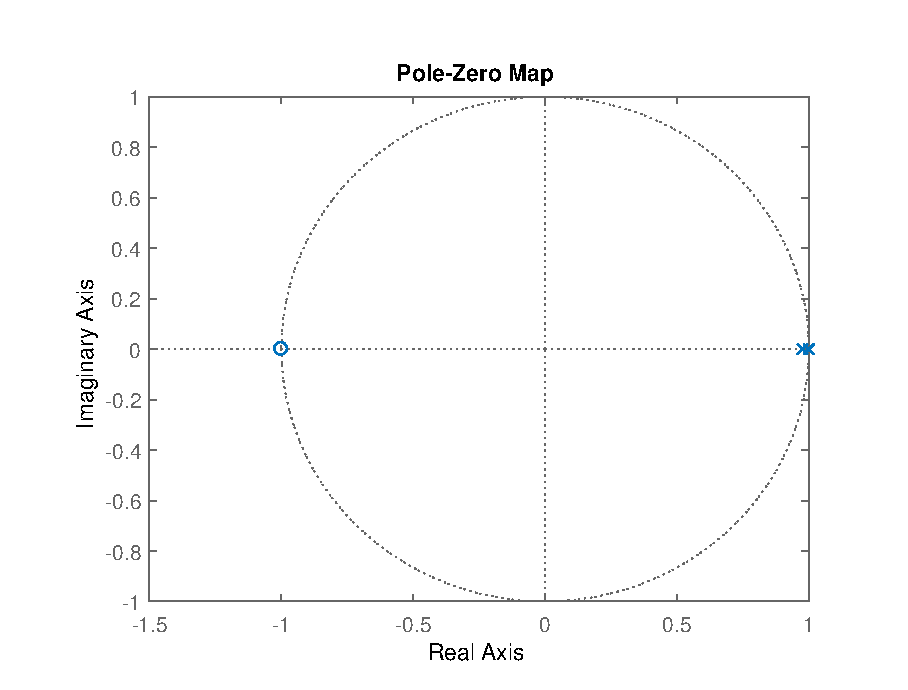
\includegraphics[width=7cm]{./img/discrete/zplot.eps}
	\caption{zplot of the new discrete system}
	\label{fig:zplot_disc}
\end{figure}

\subsubsection{Observability and controllability} 
the rank of the controllability matrix is 12 with the smallest singular value being $2.099 \cdot 10^{-3}$. The rank of the observability matrix is 12, with the smallest singular value being 4.213 $\cdot 10^{-1}$.

\subsubsection{Detectable Stabilisable}
As the system is observable this means that the system is also detectable, And as the system is controllable it is stabilisable. 

\subsubsection{minimal TODO IS THE SYSTEM MINIMUM}